\documentclass[11pt]{article}
\linespread{1.5} 
\usepackage{graphicx,epstopdf,subfigure,mathtools,mathrsfs, arydshln, amsmath, amssymb} 
\usepackage[font=small,labelfont=bf]{caption}
\usepackage{float}
\usepackage{authblk, enumitem}
\usepackage[title]{appendix}
\PassOptionsToPackage{usenames,dvipsnames}{xcolor}
\usepackage[usenames,dvipsnames]{xcolor}
\usepackage[margin=1in]{geometry}
\usepackage[normalem]{ulem}

\usepackage{amsfonts}
\usepackage{hyperref}
\hypersetup{
    colorlinks=false,
    pdfborder={0 0 0},
}
\newcommand{\new}[1]{\color{blue}#1\normalcolor}
\newcommand{\red}[1]{\color{red}#1\normalcolor}
\newcommand{\delete}[1]{}
\newcommand{\change}[1]{\color{black}#1\normalcolor}
\newcommand{\rev}[1]{\color{black}#1\normalcolor}

% VECTOR AND MATRIX NOTATION
\newcommand{\V}[1]{\boldsymbol{#1}}                 % vector notation
\newcommand{\M}[1]{\boldsymbol{#1}}
\global\long\def\norm#1{\left\Vert #1\right\Vert }
\newcommand{\Tot}[1]{#1^\text{(Tot)}}
\global\long\def\Dt{\partial_t}
\global\long\def\Dx{\partial_x}
\global\long\def\Koff{K^\text{off}}
\global\long\def\Kon{K^\text{on}}
\global\long\def\koff{k^\text{off}}
\global\long\def\koffb{\bar{k}^\text{off}}
\global\long\def\kon{k^\text{on}}
\global\long\def\Kae{K_\text{AE}}
\global\long\def\Kme{K_\text{ME}}
\global\long\def\Kem{K_\text{EM}}
\global\long\def\Kfb{K_\text{fb}}

\title{Modeling dynamics of AIR-1, ECT-2, and myosin in polarity establishment and cytokinesis \vspace{-0.5 cm}}
%\title{Mathematical appendix: \\ Oligomerization and feedback on membrane recruitment stabilize PAR-3 asymmetries in \emph{C.\ elegans} zygotes}
\author{Ondrej Maxian and Michael Glotzer \vspace{-0.75 cm}}

\begin{document}
\maketitle

\begin{abstract}
In early \emph{Caenorhabditis elegans} embryos, contractility is partially controlled by the protein ECT-2, which acts through the GTPase RhoA to activate myosin and cortical flows. Centrosomal Aurora A (AIR-1) locally inhibits ECT-2, leading to larger-scale myosin flows that amplify ECT-2 asymmetries in both polarization and cytokinesis (Longhini and Glotzer, 2022). In this study, we construct a mathematical model to determine how dynamics of ECT-2 during polarization and cytokinesis are shaped by AIR-1 and myosin. Our model, which combines a two-dimensional description of the AIR-1 profile (on the embryo cross section) with a one-dimensional description of the cortex (boundary of the cross section) demonstrates that myosin-based amplification of local AIR-1 activity is necessary to explain the cortical distribution of ECT-2 during cytokinesis. Applying the same model to polarization shows how myosin-based recruitment of ECT-2 combines with a short ECT-2 residence time to yield robust symmetry breaking.
\end{abstract}

\section{Introduction}
The anterior-posterior axis of the nematode \emph{C.\ elegans} is determined in the zygote, shortly after the egg is fertilized.  The position of sperm entry dictates the posterior pole. This event triggers myosin-dependent, anterior-directed cortical flows that facilitate the segregation of anterior and posterior PAR proteins into distinct domains \cite{munro2004cortical, lang2017proteins, gross2019guiding}.

Recent studies implicated Aurora A kinase, AIR-1, as a crucial factor required to initiate these cortical flows \cite{klinkert2019aurora,kapoor2019centrosome, longhini2022aurora}. AIR-1 associates with the sperm centrosome, which is the sperm-derived structure that promotes polarity establishment \cite{hannak2001aurora}. In recent work by Longhini and Glotzer \cite{longhini2022aurora}, it was shown that AIR-1 impacts dynamics on the cortex by inhibiting the Rho GEF ECT-2. Specifically, ECT-2 dissociates from the posterior membrane in an AIR-1 dependent manner, and it contains a consensus site for AIR-1 that is required for AIR-1 responsiveness. During polarization, ECT-2 exhibits posterior depletion and anterior enrichment; a pattern of accumulation that requires cortical myosin flows. However, unlike the anterior PAR proteins, which have residence times on the order of one hundred seconds \cite{robin2014single}, ECT-2 cannot be strongly advected, as it exchanges rapidly between the cytoplasm and the cortex on timescales of a few seconds, appearing to preferentially bind to the cortex at myosin-enriched sites \cite{longhini2022aurora}. Consequently, it remains unclear how a short residence time, preferential recruitment by myosin, and weak advection by cortical flows, could combine to generate the observed ECT-2 asymmetries during polarization. 

Longhini and Glotzer previously showed that a similar set of events occur upon anaphase onset, coincident with cytokinesis \cite{longhini2022aurora}. At first glance, these events appear quite different, as by the time cytokinesis is reached, the centrosomes have matured,  accumulated much more \mbox{AIR-1} and moved farther away from the cortex. Yet we reported a strong, ultra-sensitive dependence between the distance of the centrosome from the nearest cortical domain and the amount of cortical ECT-2 at that site; proximal centrosomes correlated with a reduction in cortical ECT-2. Because cytokinesis required myosin, it is difficult to impossible to experimentally test how the AIR-1 signal shapes the ECT-2 distribution through myosin during cytokinesis. 

In this study, we use a mathematical model to test whether the same underlying circuitry could explain the dynamics of both polarization and cytokinesis. Because our data is more abundant during cytokinesis, we choose there. We first show that the simplest model, in which AIR-1 diffuses from the centrosomes to the cortex, where it locally inhibits ECT-2, is insufficient to explain the ultra-sensitivity we observe in our previous data \cite[Fig.~7A]{longhini2022aurora}. Incorporating ECT-2 mediated activation of myosin (through Rho), plus preferential recruitment of ECT-2 by myosin, and advection of both myosin and ECT-2 through flow, then gives a closer match to our experimental data. 

Having conditioned the model (which ultimately has two unknown parameters) on cytokinesis, we then apply it to polarization \emph{without changing the parameters that govern the dynamics.} In doing so, we demonstrate that the observed dynamics of polarization and (centralspindlin-independent) cytokinesis can be explained by the same underlying model. In the context of polarization, we specifically assert that the preferential recruitment by myosin, rather than a longer bound lifetime of ECT-2, is what gives rise to the effective advection observed experimentally. 

\section{Dynamics of cytokinesis}
In previous work \cite{longhini2022aurora}, we collected a series of data on how the ECT-2 accumulation on the posterior/anterior cortex during cytokinesis depends on the position of the corresponding centrosomes. In \cite[Fig.~7A]{longhini2022aurora}, these are presented as individual embryos; here we average the individual embryos for each of the nine treatments and show the mean values (error bars are a single standard error in the mean) in Fig.\ \ref{fig:CytoSit}(a). We highlight two important aspects of this ``S-shaped'' curve: on both the anterior and posterior cortex, there is a plateau in the ECT-2 accumulation. That is, it appears that above (below) a certain distance, the ECT-2 accumulation does not depend at all on the centrosome proximity. By contrast, for distances in the range 10--20 $\mu$m, there is an ultra-sensitive dependence of the ECT-2 concentration on the proximity. Our goal in this section is to use modeling to understand these trends.

\begin{figure}
\centering
\includegraphics[width=\textwidth]{Glotzer/Fig2/Fig2-crop.pdf}
\caption{\label{fig:CytoSit} Modeling of AIR-1 signal in cytokinesis. (a) The experimental data for how the ECT-2 accumulation on the proximal cortex depends on the centrosome positions \cite[Fig.~7A]{longhini2022aurora}. Triangles are the anterior cortex, circles the posterior. Reproducing this plot via modeling is the central goal of this section. (b) Workflow for modeling the AIR-1 signal (in this case in wild-type embryos). (c) The centrosome positions for each embryo treatment, which are inputs to the diffusion model. (d) The corresponding AIR-1 signal on the cell perimeter, obtained from solving a diffusion equation. }
\end{figure}

\subsection{Solving for the AIR-1 profile}
In order to model the ECT-2 accumulation, we first need to use the centrosome locations to solve for the AIR-1 profile. Figure\ \ref{fig:CytoSit}(b) provides an overflow of this process: for each embryo type, we obtain the centrosome positions, then solve a diffusion equation to obtain the AIR-1 profile on the entire embryo cross section. Evaluating the AIR-1 concentration (which has arbitrary units) on the boundary then gives a profile on the embryo perimeter, which we flatten out to a single periodic dimension. The mathematical details of this process are discussed in Appendix \ref{sec:AIR1D}; here it suffices to list the following assumptions:
\begin{enumerate}[noitemsep, nolistsep]
\item During cytokinesis, the centrosomes have radius about 2 $\mu$m.
\item AIR-1 is activated on the centrosomes.
\item Active AIR-1 diffuses towards the cortex according to Fick's law.
\item A global phosphatase activity inactivates AIR-1 throughout the cytoplasm. 
\end{enumerate}
Setting the level of global phosphatase activity is a non-trivial undertaking. As shown in Appendix \ref{sec:AIR1D}, low levels of phosphatase activity give high global AIR-1 levels, which translate to low ECT-2 levels everywhere. Such levels were shown to block psuedocleavage in centralspindlin-independent cytokinesis, due to low contractility \cite{afshar2010regulation, kotak2016aurora}. Our choice is to set the phosphatase activity so that centrosomes close to the posterior pole (in polarization) have a negligible AIR-1 concentration in the anterior ($< 1\%$ of the anterior concentration).

\subsection{Myosin-independent models for the ECT-2 response}
Let us now examine how the strength of the AIR-1 signal affects the strength of the ECT-2 concentration on the proximal cortex. To do so, let us suppose that ECT-2 locally binds and unbinds from the cortex, with AIR-1 increasing the unbinding rate. At steady state, this gives the equation
\begin{equation}
\label{eq:EctA}
 \kon_E = \koff_E \left(1+\Kae A \right)E \rightarrow E = \frac{\kon_E/ \koff_E}{ 1+\Kae A}
\end{equation}
where $\Kae$ is the strength of AIR-1/ECT-2 inhibition, and $A_\text{min}$ is the minimum level of AIR-1 across all embryo conditions. To fit the parameters in this model, we use the AIR-1 concentration data \emph{with inactivation} (Section \ref{sec:inact}), so that the absolute concentrations are well defined. We set $\koffb=10^{-3}$ $\mu$m$^{-2}$, since this corresponds to a slight weakening of the diffusion without flattening the profile completely. This value of $\koffb$ results in the AIR-1 profiles shown in the left panel of Fig.\ \ref{fig:AIRECT}. The parameter $A_\text{min}=1.1$ is set to the minimum AIR-1 concentration across all embryos, and then $\kon_E/ \koff_E=2.5$ is obtained by fitting the maximum ECT-2 accumulation from experimental data (dhc-1 (RNAi) embryos). The last parameter $\Kae=1.3$ is set to match the minimum ECT-2 accumulation of 0.8 when AIR-1 is at its maximum (about 2.8 in dhc-1 (RNAi) embryos). The right panel of Fig.\ \ref{fig:AIRECT} shows the resulting ECT-2 profiles we obtain across different conditions. 



This model takes into account the following:
\begin{itemize}
\item ECT-2-mediated activation of myosin (through RHO-1)
\item Delayed negative feedback of myosin accumulation (through RGA-3/4-dependent inactivation of RHO-1)
\item Myosin phosphatase-dependent inactivation of myosin
\item Rapid exchange of ECT-2 at the cortex
\end{itemize}
To spatially pattern the RHO-1 dependent accumulation of myosin, we further assume:
A modest increase (2x) in the off-rate of cortical ECT-2 as a consequence of AIR-1 dependent phosphorylation of ECT-2
A modest decrease (2X) in the off rate of cortical ECT-2 due to the presence of myosin, in a myosin concentration-dependent manner.


\begin{figure}
\centering
\includegraphics[width=\textwidth]{Glotzer/Fig3/Fig3-crop.pdf}
\caption{\label{fig:LinFail}Simple models based on AIR-1/ECT-2 inhibition fail to capture the experimental data on accumulation vs.\ centrosome position. We consider (a) a linear inhibition model, and (b) a linear model with saturation (Hill function or Michaelis-Menten curve). In (i), we show the ECT-2 signal that results across the whole embryo, while (ii) isolates the signal at the anterior (triangles) and posterior (circles) cortex. Compared to the data in Fig.\ \ref{fig:CytoSit}, neither of these simple models capture the general S-shape of the curve, with plateaus at the low and high ends. }
\end{figure}

Figure\ \ref{fig:DiffCSep} compares the resulting output (right panel) to the experimental data (left panel). While we can generally reproduce the trends observed experimentally, the shape of our curve appears to be more of a line, while the experimental data show an S-shaped trend. Indeed, while we correctly predict the ECT-2 accumulation for the ``extreme'' embryos (dhc-1 (RNAi) and zyg-9 (b224)/tpxl-1(RNAi)), the intermediate embryos have A/P ECT-2 disparities which are smaller than the experimental data. For example, in wild-type embryos, the experiments show an accumulation of 1.8 on the posterior, and 1 on the anterior, while our results show an accumulation of 1.7 on the posterior and 1.4 on the anterior. 



Because we chose parameters to match dhc-1 (RNAi) embryos, their values are correct by design. If, by contrast, we had chosen a larger $K_\text{AE}$ to match wild-type embryos, then the model results would be reversed: the wild-type embryos would be correct by design, while the extreme embryos would have A/P ratios which are much \emph{larger} than the experiments. 
It seems clear that our model is missing a mechanism whereby either:
\begin{enumerate}
\item Small changes in ECT-2 concentration induced by diffusion (in an intermediate range) are amplified to become larger.
\item Large changes in ECT-2 concentration induced by diffusion are damped to become smaller.
\end{enumerate}
Since we have not accounted for the resulting actomyosin flows which tend to concentrate ECT-2, we speculate that the first of these options is what is missing from the model. We proceed to study it next.

\subsection{Flows by myosin}
We now explore the possibility that flows due to myosin could propagate smaller ECT-2 asymmetries into larger ones. To do this, we consider the basic model that ECT-2 (through activating $\rho$) activates myosin at the cortex. To minimze the number of parameters, we consider a simplified version of the true dynamics (where ECT-2 signals myosin by activating rho) and formulate a model with two variables, $E$ (for ECT-2) and $M$ (for myosin). In a system of units where length is in units of the embryo perimeter $L$, time is in units of the bound myosin lifetime $1/k^\text{off}_M$, and concentrations are scaled to be 1 when all protein is bound, the general equations governing this system can be written as
\begin{subequations}
\label{eq:MySimple}
\begin{gather}
\Dt E + \sigma_0 \Dx \left( v E\right) = D_E \Dx^2 E +\Kon_E \left(1+\Kme M\right)E_c - \Koff_E  \left(1+\Kae A\right)E \\
\label{eq:MyEq}
\Dt M + \sigma_0 \Dx \left( v M \right) = D_M \Dx^2 M +K_\text{EM} E ^2M_c - M -\Kfb M^4 \\
\label{eq:veleqn}
v = \ell^2 \Dx^2 v +\ell \Dx M \\
E_c = 1-\int_0^1 E(x) \, dx \qquad M_c = 1-\int_0^1 M(x) \, dx.
\end{gather} 
\end{subequations}
The first two equations are advection-reaction-diffusion equations which describe the dynamics of ECT-2 and myosin. The term $\sigma_0 \Dx \left(v E\right)$ describes the rate at which the ECT-2 concentration field is advected by the flow on the cortex, and likewise for the term $\sigma_0 \Dx \left(v M\right)$ in the myosin equation. In the reaction terms, we assume that myosin recruits ECT-2 from the cytoplasm, and incorporate the term $\Kme M E_c$ in the ECT-2 equation. AIR-1 inhibits ECT-2 (by promoting unbinding) according to the relationship \eqref{eq:EctA}. Myosin is locally activated at a rate proportional to \red{the square of the ECT-2 concentration (the term $\Kem E^2 M_c$; we use a squared dependence because ECT-2 asymmetries are typically 1.5:1, while myosin asymmetries are larger than 2:1, meaning there must be nonlinearity)}. We also assume delayed negative feedback of myosin via the term $\Kfb M^4$. This is an approximation of a more detailed mechanism whereby actin recruits the RhoGAPs RGA-3/4, which inactivates Rho and myosin \cite{michaux2018excitable, schmutz2007functions, schonegg2007rho}. The velocity equation\ \eqref{eq:veleqn} is a force balance equation where the active ($\Dx M$) and viscous ($\Dx^2 v$) forces are balanced by the drag force (proportional to $v$) required to drag myosin at a velocity $v$ through the cortex \cite{bois2011pattern}. The variable $\ell$ is the hydrodynamic lengthscale (approximately 10 $\mu$m \cite{mayer2010anisotropies}). 

\subsubsection{Parameter estimation}
A simple set of assumptions, some of which are based on experimental data, allows us to reduce the dynamics in\ \eqref{eq:MySimple} to two unknown parameters. We do this as follows, 
\begin{enumerate}
\item The embryo cross section is an ellipse with approximate radii 27 $\mu$m and 15 $\mu$m, which gives a perimeter $L=134.6$ $\mu$m \cite{goehring2011polarization} .
\item \red{The myosin bound lifetime is about 15 s, so $\koff_M=1/15$ s$^{-1}$. }
\item We assume that all species have a dimensional diffusion coefficient $D=0.1$ $\mu$m$^2$/s \cite{goehring2011polarization, gross2019guiding, robin2014single}. Rescaling length by $L$ and time by $\koff_M$ gives a dimensionless coefficient $D_E=D_M=0.1/(L^2 \koff_M)=4.6 \times 10^{-5}$. 
\item The ECT-2 lifetime was measured using FRAP to be on the order of a few seconds \cite{longhini2022aurora}. \red{We set $\koff_E=0.33$/s, for a three second lifetime.} Rescaling gives $\Koff_E=\koff_E/\koff_M=5$. 
\item The value of $\Kme M$ determines what fraction of ECT-2 binding occurs from recruitment by myosin. We assume that 50\% of ECT-2 is recruited by myosin, so that $\Kme M = 1$. Because $M \approx 0.3$ (see assumption 7), we set $\Kme=1/0.3$. 
%\item The value of $\Kem E$ determined what fraction of myosin activation occurs via the ECT-2 pathway. We assume that 2/3 of myosin is activated by ECT-2, so that $\Kem E=2$. Because $E \approx 0.1$ (see assumption 7), we set $\Kem=20$. 
\item We assume that 10\% of ECT-2 is bound to the cortex, and 30\% of myosin is bound to the cortex \cite[Fig.~S3j]{gross2019guiding}. This sets $\Kon_E=0.3$ and $\Kem = 50$. 
\item For the negative feedback of myosin, we use the parameters determined in \cite{michaux2018excitable}. The model there considered rho ($\rho$) and RhoGAP ($r$) as the unknowns, with the production of RhoGAP proportional to $\rho^3$ and the inhibition of $\rho$ proportional to $r \rho$. Here we coarse-grain this model into a single term, with the inhibition proportional to $M^4$. The feedback strength is obtained by assuming an equilibrium of $r$ in the equations of \cite{michaux2018excitable} (neglecting the basal binding rate), which gives (in their notation) $\Kfb=k_\text{GAP}\left(k_r^\text{ass}/k_r^\text{diss}\right)=0.1(0.245/0.047)=0.52$/s. Rescaling by $\koff_M$ gives $\Kfb=7.8$ in our model. 
\end{enumerate}
This systematic fitting procedure reduces the dynamics to two parameters: $\Kae$, which describes the rate at which AIR-1 inhibits ECT-2, and $\sigma_0$, which is the speed of flows induced by myosin gradients. By manipulating these two parameters, we can model situations where ECT-2 gradients are due to AIR-1 alone (this is Fig.\ \ref{fig:DiffCSep}, where $\Kae=1.3$ and $\sigma_0=0$), or where there is substantial amplification by flows. In the extreme case when $\Kae=0$ and $\sigma_0$ is sufficiently large, we will get oscillatory dynamics, with peaks of myosin occuring at random places, in accordance with the model of \cite{michaux2018excitable}. We need a sufficiently large $\Kae$ to ensure that the myosin peaks correspond to locations of AIR-1 depletion.

\begin{figure}
\centering
\includegraphics[width=\textwidth]{Glotzer/Fig4/Fig4-crop.pdf}
\caption{\label{fig:CytoWFlow}Incorporating flow into the AIR-1/ECT-2 model gives a better match to the experimental data. (a) Basic model of the ECT-2/Rho/Myosin circuit. (b) The corresponding data for ECT-2 accumulation vs.\ centrosome position (c.f.\ Fig.\ \ref{fig:CytoSit}(c)). (c) The dynamics of approach to steady state, starting from constant initial ECT-2 and myosin concentrations. Profiles of (i) ECT-2 concentration, (ii) Myosin concentration, and (iii) flow speed are shown from $t=0$ to $t=10$ mins, with snapshots shown every minute. Darker lines denote later times. Blue lines are dhc-1 (RNAi) embryos, while green lines denote WT. }
\end{figure}

Our approach is to start with a uniform concentration of ECT-2 and myosin, then apply the AIR-1 signal and watch the dynamics for ten minutes (long enough to reach a rough steady state, as shown in Fig.\ \ref{fig:TryFlows}). To find a combination of $\Kae$ and $\sigma_0$ that best satisfies the data, we start by fixing $\Kae$, then adjust $\sigma_0$ so that dhc-1 embryos have the experimental A/P ratio ($\approx 3.2$) of ECT-2 at the end of the simulation. We accept a pair of parameters $\left(\Kae,\sigma_0\right)$ if these same parameters give an A/P ratio around 1.8 in wild-type embryos as well. Figure\ \ref{fig:TryFlows} shows the dynamics over ten minutes with our chosen parameters $\Kae=0.5$ and $\sigma_0=0.2$. In dhc-1 embryos, there is a single peak in the ECT-2 and myosin concentration which forms at around 75\% embryo length (from the posterior), while in wild-type there are two peaks of ECT-2: one at the midline, and one at the anterior pole. 

To compare our results with flow to the experimental data, we define an accumulation on the anterior cortex as the maximum ECT-2 concentration on the anterior 25\% of the embryo length, and likewise for the posterior. Figure\ \ref{fig:ExpFlow} shows how our asymmetry results compare to the experimental data. As in the experiments, the values are taken at the time of maximum asymmetry. Compared to the previous data in Fig.\ \ref{fig:DiffCSep}, our flow-based data in Fig.\ \ref{fig:ExpFlow} show more of an ``S'' shape, qualitatively (and quantitatively, for the most part) reproducing the shape obtained in experiments.

\section{Polarization}
Here we attempt to apply our model, with the same parameters, to the process of cell polarization. We begin with the diffusion calculation to establish the profile of AIR-1, then see how this propagates in our myosin/ECT-2 model.

\subsection{Diffusion of AIR-1 \label{sec:airpol}}
In cell polarization, \emph{both} centrosomes sit very close to the posterior cortex (about 1 $\mu$m away \cite{cowan2004centrosomes}). The centrosomes have a smaller size (about 0.2 $\mu$m, so we set $\sigma_c=0.1$ $\mu$m). They also contain substantially less total AIR-1; here we assume that the amount scales with the area, so that $C_0=0.01$ for polarization. Figure\ \ref{fig:AIRPol} shows the resulting AIR-1 concentration profile (the solution of \eqref{eq:DiffEqnIn} with $\koffb=10^{-3}$ $\mu$m$^{-2}$ once again) across the embryo and along the boundary. We observe a change in AIR-1 of only 0.03 from one side of the embryo to the other, which is substantially \emph{smaller} than what we observed in cytokinesis. Considering that ECT-2 becomes asymmetrically enriched during polarization at the same levels as in cytokinesis, this underscores the need to have a mechanism to amplify the asymmetries. 

\begin{figure}
\centering
\includegraphics[width=\textwidth]{Glotzer/Fig5/Fig5-crop.pdf}
\caption{\label{fig:PolLoc}Centrosome locations set polarization dynamics. (a) The location of the centrosomes in our polarization simulations; we position both centrosomes 1, 5, and 10 $\mu$m away from the cell boundary on either the posterior pole or the cell midline. (b) The resulting AIR-1 signals along the cell perimeter. (c) The dynamics of polarization, starting from the uniform state, with the computed AIR-1 signal. Blue (purple) lines show the case when centrosomes 1 $\mu$m from the posterior pole (midline), and darker lines denote later times (0 to 10 mins). (d) Statistics on (i) ECT-2 asymmetry, (ii) myosin asymmetry, (iii) maximum flow speed, and (iv) ECT-2 clearance (measured as percentage of domain nearest the AIR-1 signal where the ECT-2 concentration is below 0.095 (see arrow in (c,i)) over time for the six centrosome locations shown in (a).}
\end{figure}

\begin{figure}
\centering
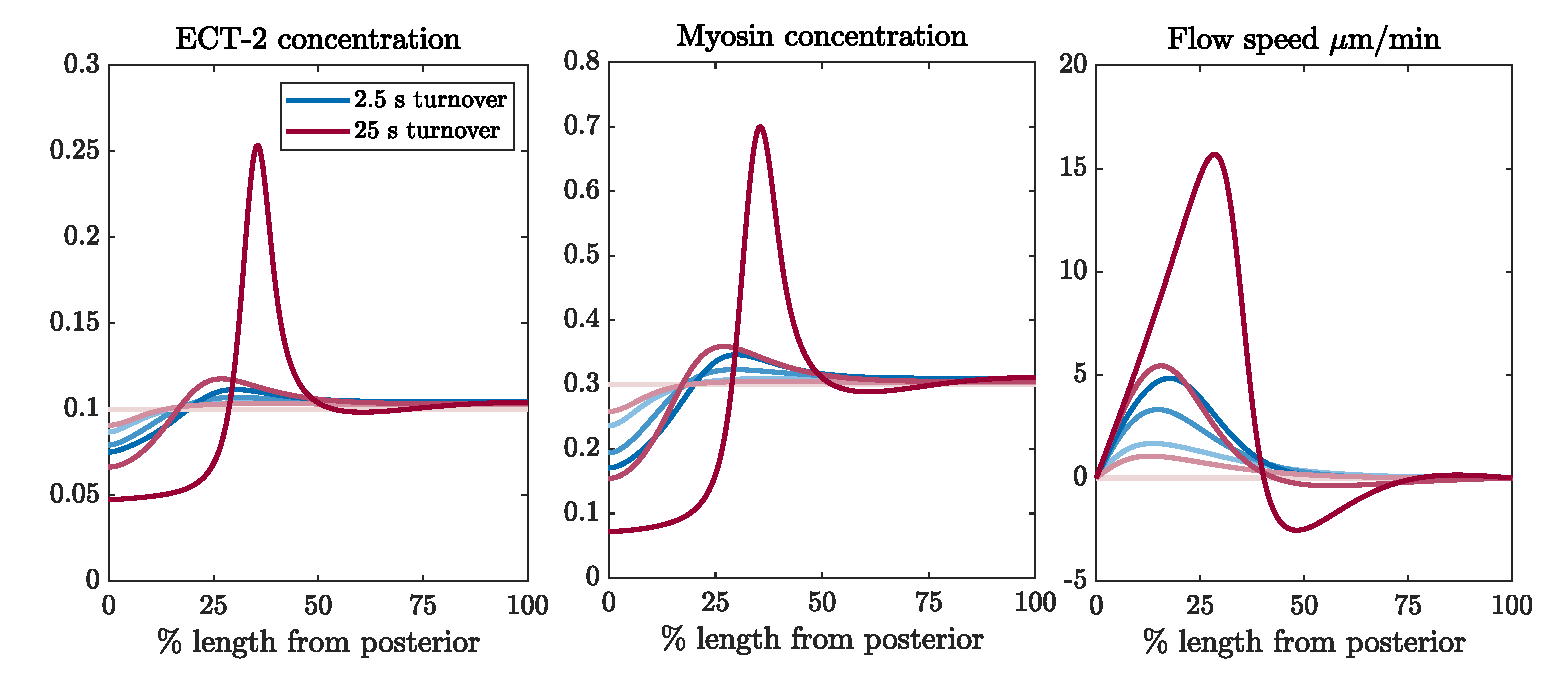
\includegraphics[width=\textwidth]{Glotzer/ECT2Residence.eps}
\caption{\label{fig:EctTurn}Fast ECT-2 turnover contributes to robust polarization dynamics. The fast turnover of ECT-2 prevents a peak forming in the middle of the cell.}
\end{figure}


\subsection{The myosin response}

We now simulate the response to the AIR-1 signal using the equations \eqref{eq:MySimple}. We use all of the same parameters as for cytokinesis, with the exception of $A_\text{min}$, which is the ``base'' concentration of AIR-1, at which there is no effect on ECT-2. We previously set this value to be the smallest value of the AIR-1 concentration across all embryos in cytokinesis; here we use the minimum concentration for polarization, which, according to Fig.\ \ref{fig:AIRPol} is $A_\text{min}=0.01$. 


\red{Figure \ref{fig:TryFlowsPol} shows the response of the system to the AIR-1 signal, which in polarization is highly localized to the posterior cortex (see Fig.\ \ref{fig:AIRPol}). In the first ten minutes of simulation time (which is longer than polarity establishment phase), a peak in myosin and ECT-2 forms immediately next to the posterior pole as a result of depletion of ECT-2 there. Following this, the higher ECT-2 concentration pulls in some ECT-2 from the anterior, which leads to a counter-flow, local depletion of ECT-2 next to the peak, and another smaller peak next to the first at steady state. If the domain were longer, this process would keep propagating, with smaller and smaller peaks forming in the anterior. Note also that the low residence time of ECT-2 prevents a larger flow from the anterior into the peak, which leaves the anterior concentration at a higher level than the posterior.}


\subsubsection{Trying a larger AIR-1 signal}

\red{In Fig.\ \ref{fig:TryFlowsPolQ}, we demonstrate what happens when the AIR-1 signal is larger on the posterior pole. Specifically, we repeat the entire process, from the diffusion to polarization calculation, with the centrosomes having four times as much AIR-1. The result is that the ECT-2 concentration on the posterior pole drops even lower than previously observed. This drives a larger flow towards the anterior, which pushes the ECT-2 and myosin peak towards the middle of the embryo. The peak in the middle of the embryo then prevents the second peak from forming in the domain interior. The larger flow also leads to the steady state being assumed quite rapidly. }

\begin{appendix}
\section{Mathematical appendix} 

\subsection{AIR-1 diffusion model \label{sec:AIR1D}}
The contractility circuit is forced by a cue from the centrosomes which contain Aurora A (AIR-1), an inhibitor of ECT-2. We assume that the AIR-1 signal gets to the membrane by diffusion. Letting $a(\V x)$ be the concentration of AIR-1 in the embryo, we have the equation
\begin{subequations}
\label{eq:CD}
\begin{gather}
\label{eq:DiffEqn}
\Delta a -\koffb a=  -f \qquad \V{x} \in \Omega.\\
\label{eq:DiffBC}
\nabla a \cdot \V{n}=0 \quad \V{x} \in \partial \Omega,
\end{gather} 
where\ \eqref{eq:DiffEqn} is the diffusion equation for the concentration and\ \eqref{eq:DiffBC} is a no-flux boundary condition through the boundary (here $\Omega$ represents the embryo area and $\partial \Omega$ represents the boundary). The signal $f(\V x)$ comes from the two centrosomes, which we model by Gaussian densities 
\begin{equation}
f(\V{x}) = \frac{C_0/D}{2 \pi \sigma_c^2}\sum_{i=1}^2\exp{\left(\frac{-\norm{\V{x}-\V{x}_i}^2}{2 \sigma_c^2}\right)}.
\end{equation}
Here $\V{x}_i$ is the location of the $i$th centrosome (typically at some location $(x_i,0)$), which changes depending on the embryo conditions. In addition to the centrosome location, the signal has two other parameters: $C_0/D$ is the strength of the cue (the integral of $f(\V{x})$ over the entire embryo cross-section, normalized by the cytoplasmic diffusion coefficient $D$), and $\sigma_c$ is the centrosome ``size'' (the standard deviation of the Gaussian, which is roughly half the size of the centrosome). For cytokinesis, the centrosomes have size about 2 $\mu$m, so we set $\sigma_c=1$ $\mu$m.
\end{subequations}
The diffusion equation\ \eqref{eq:DiffEqn} also contains a basal rate of inactivation of AIR-1 (phosphatase activity). This introduces another parameter which is the inactivation rate relative to the diffusion coefficient in the cytoplasm ($\koffb$, units $\mu$m$^{-2}$). 

We use a standard first-order finite element method to solve\ \eqref{eq:DiffEqn}. In brief, the elliptical domain of the embryo is meshed into nodes and triangles, which define a set of linear Lagrangian basis functions $\psi_k$ that are 1 at node $\V{x}_k$ and 0 everywhere else. Multiplying\ \eqref{eq:DiffEqn} by a basis function $\psi_k$, then integrating by parts using the boundary condition\ \eqref{eq:DiffBC} gives 
\begin{equation}
\sum_j \int_{\Omega} \left(\nabla \psi_k \cdot \nabla \psi_j\right) a_j \, d\V{x}+\sum_j \int_{\Omega} \psi_k \psi_j a_j \, d\V{x}= \sum_j \int_{\Omega} \psi_k \psi_j f_j \, d\V{x},
\end{equation}
which can be written as the matrix equation $\left(\M K + \koffb \M M \right) \V a = \M M \V f$, where $\M{M}$ is the so-called mass matrix and $\M{K}$ the stiffness matrix for finite elements. 

To constrain the level of phosphatase activity (parameter $\koffb$), we compute the profile of AIR-1 under polarization conditions (both centrosomes 1 $\mu$m from the posterior pole, with $C_0/D=0.01$), and plot the resulting AIR-1 signal in Fig.\ \ref{fig:AIR1ProfKoff}. When the phosphatase activity is low, the no flux boundary condition traps AIR-1 inside the embryo, and the relative difference between posterior and anterior is small. Increasing the phosphatase activity disproportionately lowers AIR-1 levels on the anterior pole (since it is much farther from the centrosomes). We assume that anterior levels of AIR-1 during polarization are at most 1\% of posterior levels; this constrains $\koffb=10^{-2}$. 

\begin{figure}
\centering
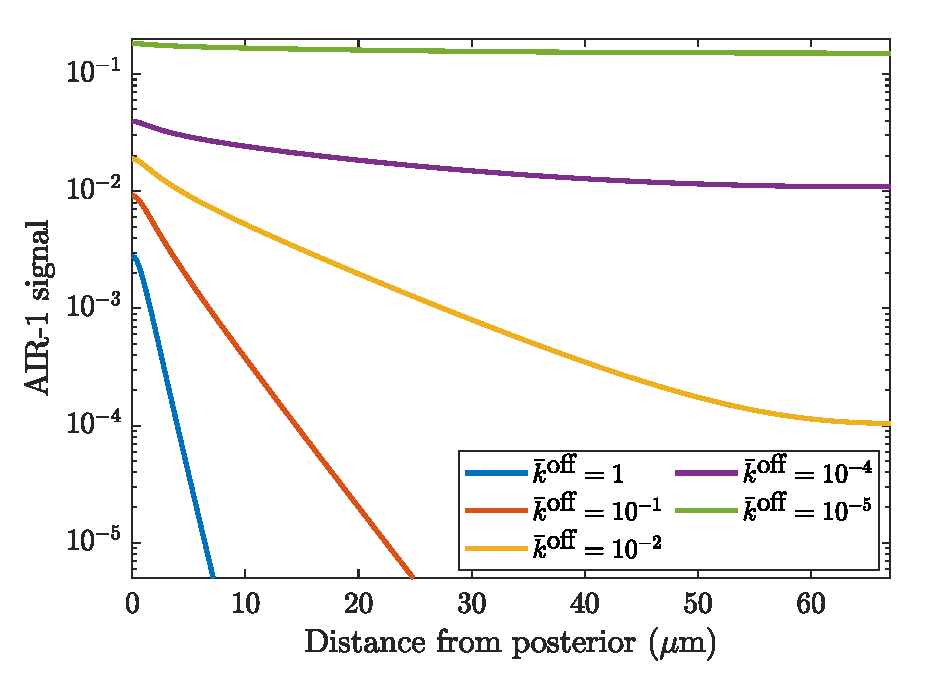
\includegraphics[width=0.6\textwidth]{Glotzer/PolarizationKoffAir.eps}
\caption{\label{fig:AIR1ProfKoff}AIR-1 signal vs.\ distance from posterior under polarization conditions (blue squares in Fig.\ \ref{fig:PolLoc}(a)). We vary the level of phosphatase activity $\koffb$ until the posterior level is less than 1\% of the anterior level, settling on $\koffb=10^{-2}$ $\mu$m$^{-2}$.}
\end{figure}

\subsection{ECT-2/Myosin circuit}

\end{appendix}

\bibliographystyle{plain}

\bibliography{../../PolarizationBib}


\end{document}
